\documentclass[10pt, a4paper]{article}

% Import the packages
\usepackage[utf8]{inputenc}
\usepackage[english, spanish]{babel}
\usepackage[left=25mm, right=25mm, top=35mm, bottom=30mm, headheight=35mm]{geometry}
\usepackage{graphicx}
\usepackage{float}
\usepackage{xcolor}
\usepackage{fancyhdr}
\usepackage{hyperref}
\usepackage{setspace}
\usepackage{indentfirst}

% Syntax customization with minted package
\usepackage{minted}
\usemintedstyle{nord-darker}
\setminted{
  breaklines,
  linenos,
  frame=lines,
  fontsize=\normalsize
}
\newcommand{\mpy}[1]{\mintinline[style=gruvbox-light]{python}{#1}}

% Define background color
\definecolor{background}{HTML}{2E3440}

% Variables
\newcommand{\university}{Universidad Nacional de San Agustín de Arequipa}
\newcommand{\faculty}{Facultad de Ingeniería de Producción y Servicios}
\newcommand{\program}{Escuela Profesional de Ingeniería de Sistemas}
\newcommand{\semester}{2024 - A}
\newcommand{\course}{img/web_programming.png}
\newcommand{\topic}{img/opp_with_python.png}
\newcommand{\professor}{Quispe Cruz, Marcela}
\newcommand{\students}{Arias Quispe, Jhonatan David\\Mamani Huarsaya, Jorge Luis\\Velarde Saldaña Jhossep Fabritzio} 
\newcommand{\github}{https://github.com/jorghee/OOP-with-python}
\newcommand{\mydate}{28 de mayo, 2024}

% Just parts and chapters numbered
\setcounter{secnumdepth}{0}

% Head and foot customization
\pagestyle{fancy}
\lhead{\raisebox{-0.2\height}{
\includegraphics[width=4cm]{img/logo_unsa.png}}}
\chead{\fontsize{8}{8}\selectfont \university \\ \faculty \\ \textbf{\program}}
\rhead{\raisebox{-0.2\height}{
\includegraphics[width=3.5cm]{img/logo_episunsa.png}}}
\lfoot{Semestre \semester}
\cfoot{}
\rfoot{Pág. \thepage}

\begin{document}

\begin{titlepage}
	\centering
	\includegraphics[width=15cm]{\course} \par
  \vfill \vfill
	\includegraphics[width=15cm]{\topic}\par
  \vfill \vfill
  {\textbf{Profesor(a):} \par}
	\professor \vfill
  {\textbf{Estudiantes:} \par}
	\students \vfill
  {\textbf{Repositorio GitHub:} \par}
  \href{\github}{\github} \vfill
	{\large \mydate \par}
\end{titlepage}

\section{El programa Agenda telefónica}

\begin{itemize}
  \item El programa necesita guardar los datos que el usuario dispone, estos datos deben ser almacenados en algún tipo de archivos. Debido a que se necesitan guardar listas de objetos, se ha decidido hacer uso de archivos JSON, un formato ligero de intercambio de datos, fácil de leer y escribir con la biblioteca json de Python, adecuado para datos estructurado.
  \item Leer y escribir en archivos con Python viene de forma nativa y se utiliza a través de las funciones integradas \mpy{open}, \mpy{read}, \mpy{write} entre otras. Sin embargo para manejar ciertos formatos especificos como JSON, Python ofrece el modulo estándar json.
\end{itemize}

\subsection{La clase Contacto}
Contiene los campos mencionados necesarios para identificar al contacto

\begin{minted}[bgcolor=background]{python}
def __init__(self, nombre: str, telefono: str, direccion: str, relacion: str):
  self._nombre = nombre
  self._telefono = telefono
  self._direccion = direccion
  self._relacion = relacion
\end{minted}

Además debe de contener los métodos que se llaman automaticamente al momento de representar como string al objeto actual.

\begin{minted}[bgcolor=background]{python}
def __repr__(self) -> str:
  return self.__str__()

def __str__(self) -> str:
  return (f"\nNombre:\t\t{self._nombre}\nTelefono:\t{self._telefono}\n"
          f"Direccion:\t{self._direccion}\nRelacion:\t{self._relacion}\n")
\end{minted}

Debemos de tener un método que nos permita parsear el objeto actual como un diccionario. Por ejemplo, que el identificador de referencia al campo name sea como clave y su valor sea el correspondiente valor del campo.

\begin{minted}[bgcolor=background]{python}
def parsear_a_json(self):
  return {
    "nombre": self.nombre,
    "telefono": self.telefono,
    "direccion": self.direccion,
    "relacion": self.relacion
  }
\end{minted}

Un método que reciba como argumento un diccionario, basicamente es el objeto JSON parseado por el modulo json de Python. Este diccionario contiene los campos de una instancia de la clase Contact, por lo tanto con estos datos se debe crear el nuevo objeto. Si analizamos, este método será parte de cargar los datos guardados en un archivo JSON.

\begin{minted}[bgcolor=background]{python}
@staticmethod
def parsear_de_json(dic):
  return Contacto(dic["nombre"], dic["telefono"], dic["direccion"], dic["relacion"])
\end{minted}

El método debe de ser estático porque necesitamos acceder a este mismo sin tener que crear aún un objeto Contacto.

\subsection{La clase Agenda}
Esta clase contiene un campo \mpy{self._contacts} que es una lista de objetos Contacto. Aqui tenemos una particularidad a destacar. Se decidió que el \textbf{archivo que guarda los contactos se recupera automáticamente} al momento de crear una instancia de esta clase.

\begin{minted}[bgcolor=background]{python}
def __init__(self, path_data):
  self._contacts = self.recuperar_agenda(path_data)
\end{minted}

Por lo tanto, comenzaremos explicando el método \mpy{recuperar_agenda()}.

\subsubsection{El método \mpy{recuperar_agenda(path_data)}}
La lógica es recuperar el archivo con la dirección que nosotros como desarrolladores han decidido, en caso no exista el archivo, entonces se regresa una lista vacíá; de lo contrario necesitamos cargar el archivo.

\begin{minted}[bgcolor=background]{python}
def recuperar_agenda(self, path_data):
  if not (os.path.exists(path_data)):
    return []

  with open(path_data, "r") as data: 
    datos = json.load(data)
    print("Recuperación exitosa...\n")
  return [Contacto.parsear_de_json(dic) for dic in datos]
\end{minted}

Cuando cargamos el archivo, este se carga en diccionarios, ya que la conversión de objetos JSON es a diccionarios en Python. Entonces aqui debemos de utilizar el método \mpy{parsear_de_json()} que recibe el diccionario y crear con estos valores el objeto Contacto. 

\subsubsection{El método \mpy{getContact(pattern)}}
Básicamente la lógica consiste en iterar sobre las lista \mpy{self._contacts} y recuperar su campo \mpy{nombre}.
\singlespacing
Ahora necesitamos comparar dicho nombre con el patrón ingresado. Para resolver este problema se ha utilizado el siguiente algoritmo.

\paragraph{Algoritmo de Knuth-Morris-Pratt (KMP):}
El algoritmo KMP utiliza la información del propio patrón para evitar retrocesos innecesarios en la cadena de texto. Esto se logra mediante la construcción de un arreglo de prefijo (función de prefijo o función $\pi$), también conocido como "arreglo de fallos" o "tabla de fallos", que se utiliza para saltar comparaciones redundantes.

\begin{figure}[H]
  \centering
  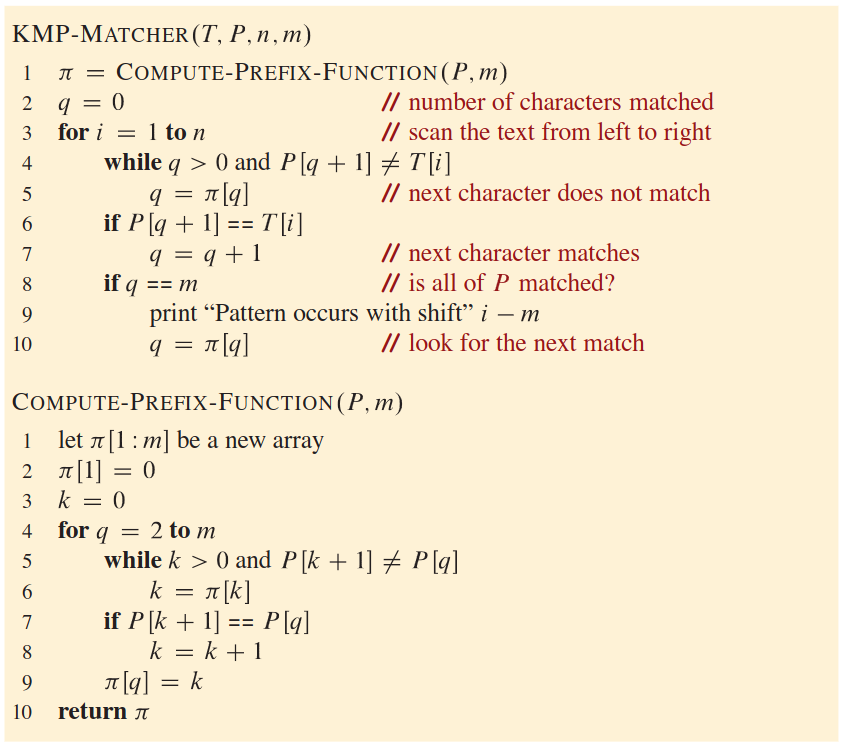
\includegraphics[width=0.8\textwidth]{img/kmp.png}
  \caption{Pseudocodigo del algoritmo KMP}
\end{figure}

Entonces en ves de devolver el indice de la primera posición de la cadena de texto de todas las coincidencias, nosotros hemos hecho que devuelva \mpy{True} o \mpy{False}.


\begin{minted}[bgcolor=background]{python}
# Algoritmo Knuth-Morris-Pratt (KMP)
def _match(self, name, pattern):
  lps = self._compute_lps(pattern)
  i = 0
  j = 0

  while i < len(name):
    if pattern[j] == name[i]:
      i += 1
      j += 1

    if j == len(pattern):
      j = lps[j - 1]
      return True
    elif i < len(name) and pattern[j] != name[i]:
      if j != 0:
        j = lps[j - 1]
      else:
        i += 1
  return False

# Generación de la funcion $\pi$
def _compute_lps(self, pattern):
  lps = [0] * len(pattern)
  length = 0
  i = 1

  while i < len(pattern):
    if pattern[i] == pattern[length]:
      length += 1
      lps[i] = length
      i += 1
    else:
      if length != 0:
        length = lps[length - 1]
      else:
        lps[i] = 0
        i += 1
  return lps
\end{minted}

\subsubsection{El método \mpy{guardar_agenda()}}
El método consiste en iterar en los objetos de la lists \mpy{self._contacts} y generar una lista ya no de objetos Contacto, sino ahora una lista de diccionarios, usando el método \mpy{parsear_a_json()} de la clase Contacto.

\begin{minted}[bgcolor=background]{python}
def guardar_agenda(self):
  contacts_pars = [contact.parsear_a_json() for contact in self._contacts]
  with open("./data/data.json", "w", encoding = "utf-8") as save:
    json.dump(contacts_pars, save, ensure_ascii=False, indent=2)
    print("Guardacion exitosa...\n")
\end{minted}

\subsection{Método \texttt{updateContact}}
\subsubsection{Definición del Método}
\begin{verbatim}
\begin{lstlisting}[language=python]
def updateContact(self, newContact):
    for idx, saved in enumerate(self._contacts):
        if saved.nombre == newContact.nombre:
            self._contacts[idx] = newContact
            print("El contacto se actualizó exitosamente...\n")
            return
    print("No se encontró el contacto a actualizar...\n")
\end{lstlisting}
\end{verbatim}

\subsubsection{Descripción del Funcionamiento}
\begin{itemize}
    \item \textbf{Propósito:}
    Actualizar un contacto existente en la lista \texttt{\_contacts}.
    \item \textbf{Parámetros:}
    \texttt{newContact}: Un objeto de contacto que contiene la nueva información que se desea actualizar.
    \item \textbf{Flujo de Control:}
    \begin{itemize}
        \item \textbf{Iteración:} El método recorre la lista \texttt{\_contacts} usando \texttt{enumerate} para obtener tanto el índice como el objeto de contacto actual.
        \item \textbf{Comparación:} Dentro del bucle, compara el nombre (\texttt{nombre}) del contacto guardado (\texttt{saved}) con el nombre del nuevo contacto (\texttt{newContact}).
        \item \textbf{Actualización:} Si encuentra una coincidencia, reemplaza el contacto existente en la lista con el nuevo contacto (\texttt{newContact}).
        \item \textbf{Salida:} Imprime un mensaje de éxito y sale del método con \texttt{return} para evitar iteraciones innecesarias.
        \item \textbf{No Encontrado:} Si no se encuentra una coincidencia tras iterar toda la lista, imprime un mensaje indicando que no se encontró el contacto.
    \end{itemize}
\end{itemize}

\subsection{Método \texttt{deleteContact}}
\subsubsection{Definición del Método}
\begin{verbatim}
\begin{lstlisting}[language=python]
def deleteContact(self, pattern):
    for contact in self._contacts:
        name = contact.nombre
        isName = self._match(name.lower(), pattern.lower())
        if isName:
            self._contacts.remove(contact)
            print("El contacto se eliminó exitosamente...\n")
            return
    print("No se encontró el contacto a eliminar...\n")
\end{lstlisting}
\end{verbatim}

\subsubsection{Descripción del Funcionamiento}
\begin{itemize}
    \item \textbf{Propósito:}
    Eliminar un contacto de la lista \texttt{\_contacts} que coincida con un patrón dado.
    \item \textbf{Parámetros:}
    \texttt{pattern}: Un patrón de texto que se usará para buscar coincidencias en los nombres de los contactos.
    \item \textbf{Flujo de Control:}
    \begin{itemize}
        \item \textbf{Iteración:} El método recorre la lista \texttt{\_contacts}.
        \item \textbf{Comparación:} Convierte los nombres de los contactos y el patrón a minúsculas para una comparación insensible a mayúsculas/minúsculas.
        \item \textbf{Coincidencia:} Utiliza un método auxiliar \texttt{\_match} para verificar si el nombre coincide con el patrón.
        \item \textbf{Eliminación:} Si encuentra una coincidencia, elimina el contacto de la lista \texttt{\_contacts}.
        \item \textbf{Salida:} Imprime un mensaje de éxito y sale del método con \texttt{return}.
        \item \textbf{No Encontrado:} Si no se encuentra una coincidencia tras iterar toda la lista, imprime un mensaje indicando que no se encontró el contacto.
    \end{itemize}
\end{itemize}
\section{El programa Carrito de Compras}
\subsection{La clase ProductStock}
Por el momento solo contiene los 3 campos name, value y quatity, además de su correspondiente constructor y los métodos setters y getters.

\begin{minted}[bgcolor=background]{python}
class ProductStock:
  def __init__(self, name, value, quantity):
    self._name = name
    self._value = value
    self._quantity = quantity
\end{minted}

\subsection{La clase StockProducts}
Contiene un campo que almacena los productos en stock. Por lo tanto puede ser una lista de objetos ProductStock, sin embargo, podemos especificar un id para cada tipo de producto, una forma de identificarlo unicamente y que con id directamente podamos acceder a la informacion del producto como es el nombre, costo y cantidad.

\subsubsection{Qué estructura usar}
Los diccionario en Python nos facilitaria acceder directamente a la informacion del producto sin la necesidad de tener que iterar por cada objeto ProductStock y comparar su campo name como se tendria que hacer si la estructura sería una simple lista de objetos ProductStock.

\begin{minted}[bgcolor=background]{python}
class StockProducts:
  def __init__(self):
    self._products = {}
\end{minted}

\subsubsection{El método \mpy{add_product()}}
Se encargará de agregar un nuevo producto al diccionario, donde la clave es el nombre del producto, asi ingresar a la información del producto es más eficiente.

\begin{minted}[bgcolor=background]{python}
def add_product(self, product):
  self._products[product.name] = product
  print("Producto agregado en stock exitosamente...")
\end{minted}

\subsubsection{El método \mpy{get_product()}}
Se encargará de obtener el producto según el nombre que reciba como argumento, aqui podemos observar la funcionalidad del diccionario, ya que solo necesitamos pasar el argumento como clave para buscar en el diccionario en vez de tener que iterar por cada objeto en caso de una lista. Claro esta que son estructuras de datos y su concepto no involucra saber cómo esta implementado por dentro.

\begin{minted}[bgcolor=background]{python}
def get_product(self, name):
  return self._products.get(name)
\end{minted}

Como vemos, solo consta en usar la función \mpy{get()} en lugar de acceder nativamente al valor del diccionario. Si nosotros usamos esta forma, entonces si en futuras verificaciones como es en el caso de la clase \textbf{ShoppingCart} puede arrojar un error al no encontrar dicha clave.

\subsubsection{El método \mpy{delete_products()}}
Este método es usado en el método \mpy{finalize_purchase()} de la clase \textbf{ShoppingCart}. Se encarga de reducir la cantidad de unidades disponibles de cada producto que esta en stock.

\begin{minted}[bgcolor=background]{python}
def delete_products(self, name, cuantity):
  if self._products[name].cuantity >= cuantity:
    self._products[name].cuantity -= cuantity 
    print("Producto eliminado exitosamente...")
  else:
    print("Producto no encontrado...")
\end{minted}

\subsection{La clase ShoppingCart}
Al igual que la clase StockProducts usamos el concepto de \textbf{Asociación}, pues se tendrá una referencia una instancia de StockProducts, lo cual nos permite saber la informacion de la lista de productos en stock, claro está que es un diccionario.

\subsubsection{Almacenar los productos y la cantidad de unidades en el carrito de compras}
Para poder conectar con los productos en stock rápidamente podemos pensar que esta estructura tambien debe de ser un diccionario donde la clave es el nombre del producto y el valor es la cantidad de unidades puestas en el carrito de compras

\begin{minted}[bgcolor=background]{python}
class ShoppingCart:
  def __init__(self, stock):
    self._stock = stock   # Productos en stock
    self._item = {}   # Productos en el carrito
\end{minted}

\subsubsection{El método \mpy{add_item()}}
Como vemos, este método debe de recibir 2 argumentos, que son el nombre del producto y la cantidad de unidades a comprar. Entonces la lógica en este método se divide en 2 partes:

\begin{itemize}
  \item Verificar si el producto está en el campo que referencia a una instancia de StockProducts y verificar tambien si la cantidad a comprar es menor o igual que la cantidad disponible.
  \item Verificar que si el el producto ya está en el carrito de compras solo aumentar la cantidad de unidades, de lo contrario agregar el producto al carrito de compras con su correspondiente cantidades de unidades iniciales.
\end{itemize}



\end{document}
